\documentclass[11pt,a4paper]{scrreprt}
% Basispakete
\usepackage[pdftex]{hyperref}                   % Links
\usepackage[utf8]{inputenc}                     % Typesetting
\usepackage{ngerman}                            % Deutsche Silbentrennung
\usepackage{amsmath}                            % AMS Math
\usepackage{amssymb}                            % AMS Math
\usepackage[automark]{scrpage2}                 % scrpage
\usepackage{graphicx}                           % Grafiken
\usepackage{makeidx}                            % Inhaltsverzeichnis
\usepackage{ulem}                               % Durchgestrichener Text

% Hyperref konfigurieren
\hypersetup{
    unicode=false,          % non-Latin characters in Acrobat’s bookmarks
    pdftoolbar=true,        % show Acrobat’s toolbar?
    pdfmenubar=true,        % show Acrobat’s menu?
    pdffitwindow=false,     % window fit to page when opened
    pdfstartview={FitH},    % fits the width of the page to the window
    pdftitle={My title},    % title
    pdfauthor={Author},     % author
    pdfsubject={Subject},   % subject of the document
    pdfcreator={Creator},   % creator of the document
    pdfproducer={Producer}, % producer of the document
    pdfkeywords={keyword1} {key2} {key3}, % list of keywords
    pdfnewwindow=true,      % links in new window
    colorlinks=false,       % false: boxed links; true: colored links
    linkcolor=red,          % color of internal links
    citecolor=green,        % color of links to bibliography
    filecolor=magenta,      % color of file links
    urlcolor=cyan           % color of external links
}

% Seitenstil scrheadings verwenden
\pagestyle{scrheadings} 

% Grösse des Textbereiches in der Seite
\setlength{\textwidth}{15cm}
\setlength{\textheight}{21cm}

% Kopf- und Fusszeile, Höhe und Abstand vom Text
\setlength{\headheight}{15pt}
\setlength{\headsep}{0.8cm}

% Linker Seiteneinzug
\setlength{\oddsidemargin}{2.5cm} \addtolength{\oddsidemargin}{-1in}
\setlength{\evensidemargin}{2.5cm} \addtolength{\evensidemargin}{-1in}

% Andere Grössen ausrechnen (vertikal zentrieren)
\setlength{\footskip}{\headsep}
\addtolength{\footskip}{\headheight}
\setlength{\topmargin}{\paperheight}
\addtolength{\topmargin}{-\textheight}
\addtolength{\topmargin}{-\headheight}
\addtolength{\topmargin}{-\headsep}
\addtolength{\topmargin}{-\footskip}
\addtolength{\topmargin}{-2in}
\addtolength{\topmargin}{-0.5\topmargin}

% Sektion und Kapitel für Headmark
\automark[section]{chapter} 

% Separate Linie im Kopf
\setheadsepline{.4pt} 
% Kopf und Fußzeile löschen
\clearscrheadfoot

% linke Kopfzeile 
\ihead[\headmark]{\headmark}

% mittlere Fusszeile 
\cfoot[\pagemark]{\pagemark}

\title{Lernmodul Process Scheduling}
\author{Vorlesung Betriebssysteme UniBe}
\date{März 2012}

\makeindex

\begin{document}

\maketitle
\tableofcontents
\newpage

\section*{Vorwort}
Dieses Dokument soll eine Kopie des Kurses \textit{Lernmodul Process Scheduling} bieten. Der Inhalt ist nicht von mir, sondern aus dem erwähnten Modul. \\
Minimale Korrekturen betreffen die folgenden Punkte:
\begin{itemize}
\item Tests, welche nicht gemacht werden sollen, wie ''My Goals'' und die im Kapitel 4 (''Personal Synthesis'', ''Survey'') wurden gemäss Besprechung entfernt.
\item Um der Gliederung in Folien Rechnung zu tragen, wurden zusätzliche Überschriften eingefügt. Diese wurden kursiv markiert.
\item Formatierungsfehler wurden korrigiert (z.B. $\backslash$222 zu ', fehlende Leerzeichen), leere Seiten und Abschnitte wurden entfernt.
\item Die Formeln wurden neu gesetzt.
\end{itemize}

\section*{Kurzzusammenfassung Übungsstunde}
\textit{Process Scheduling} ist eines der beiden Module, die im Kurs Betriebssysteme anfallen (das andere wird später \textit{File Systems} sein). Der Kurs ist auf \textbf{ILIAS} zugänglich. Geschätzter Aufwand ca. 22.5h. \\
\textbf{Abgabe}: Bis 16.04.2012, praktischer Teil per Email an \href{mailto:wagen@iam.unibe.ch}{Gerald Wagenknecht}.\\\\
Zu erledigende Quizzes und Tests:
\begin{itemize}
\item Self Test (0p), Einschätzung
\item Quiz (30p), Theorie
\item ''Final Quiz'' (40p), Abgabe der Programmieraufgabe
\end{itemize}
Implementierung in Java mit Hilfe des PSSimulators, mit Template \href{https://ilias.unibe.ch/repository.php?ref_id=402886&cmd=sendfile}{\texttt{ps\_template.zip}}.

\chapter{Introduction}
Process scheduling is the primary task of any modern operating system to handle multi tasking. Early operating systems did not offer multi tasking though, but the outstanding growth of CPU power as well as the development of thousands of applications and tools possibly used concurrently rapidly underlined the need of efficient process scheduling by the operating system. In this module, students learn about processes and scheduling processes under limited resources (CPU, memory, disks and other IO devices, ...). They also acquire knowledge on how theprocess scheduler of the operating system actually achieve its task. In order to apply their knowledge, the students implement severalscheduling algorithms inside a simulator.

\section{Special Requirements}
\begin{itemize}
\item Basic knowledge of the Java programming language.
\end{itemize}

\section{Author}
The module ''Process Scheduling'' has been created by \textit{Frederic Aubert} and \textit{Randoald Corfu}, University of Neuchâtel. \\\\
For further conceptual information regarding the module ''Process Scheduling'' please contact \textit{frederic.aubert@unine.ch}.

\section{Goals}
\begin{itemize}
\item You study the concepts of process and process states.
\item You learn about process scheduling and different algorithms in use.You have to pass the Self-test with no wrong answer, in order to prepare for the Quiz. The Quiz will be scored by your tutor.
\item You apply your knowledge by implementing three scheduling algorithms insidea simulator. You perform actual simulation with given input, in order to compute specific statistics that you will be asked to comparatively discuss. Your written code as well as your comparative discussion will be evaluated by your tutor.
\end{itemize}

\newpage

\section{Schedule}
\begin{figure}[!ht]
\centering
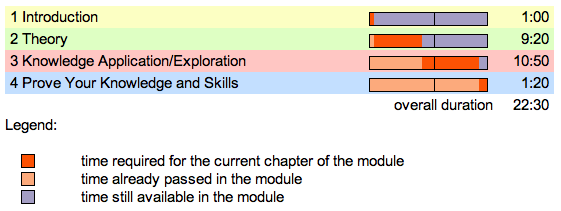
\includegraphics[width=0.8\linewidth]{img/schedule.png}
\end{figure}

\chapter{Theorie}
\section{\textit{Introduction}}
When using any modern computer, we often have the feeling that more than one program is executed at the same time. However this is not the case, since the processor, the key unit that executes the instructions of a program, can only handle one instruction at a time. In the reality, the processor swaps between all programs, allocating in turns a time slot to each of them during which some but not necessarily all instructions are executed. These time slots are small enough to give to the user an illusion of parallelism. We say that such Operating System handle multi tasking. \\\\
True parallelism can of course be achieved on multiprocessor computers. But even on such architectures, we often face the challenge that we have more programs in execution than we have processors in the machine. We again are in need of multi tasking. Furthermore since the memory is usually shared by all processors, the management of all parallel activities become even more complex.
\newpage
To address the multi tasking issue, the early developers of operating systems formulated a model based on independent \textit{sequential processes} operating in a \textit{multiprocessor environment}. \textit{Sequential process}, also simply called \textbf{process}, consists of a program in execution to which is associated a program counter, some registers, and a pool of memory which holds the content of program variables. Conceptually each \textbf{process} has its own \textit{virtual processor}. It shouldn’t have to worry about whether it is going to be executed on a single processor or on a multiprocessor computer.
\begin{figure}[!ht]
\centering
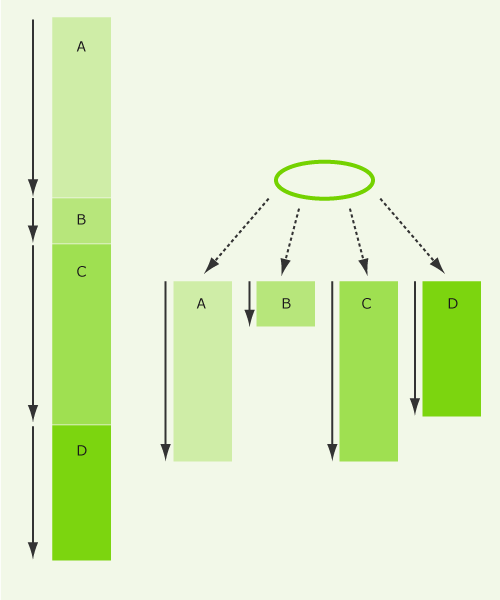
\includegraphics[width=0.7\linewidth]{img/process1.png}
\caption{Figure 1}
\label{fig:figure1}
\end{figure} 
\clearpage
Let's consider that we have four processes, A, B, C, and D as shown in figure \ref{fig:figure1}. For a process to be executed, all instructions need to be executed, from the first one to the last one. On the left side, the four processes are executed one after the other, sequentially, on a single processor computer. There is no multi tasking. On the right side, the four processes are executed simultaneously, on a multiprocessor computer that has at least four processors. The multiprocessor architecture provides multi tasking by itself. \\\\
Now let's imagine we have a dual processor computer. On the left side, the four processes are executed sequentially and independently on the two processors. When one process terminates, the next one takes its place. Here again the multiprocessor architecture provides multi tasking by itself. On the right side, the four processes are sliced into small fragments, which are then executed sequentially. When one fragment terminates, the next one takes it place. This rule allows for example a process to start on processor I, pass twice on processor II, and finish on processor I. Here, the time slot mechanism provides multi tasking. We can finally notice that multi tasking decreases global execution time.
\begin{figure}[!ht]
\centering
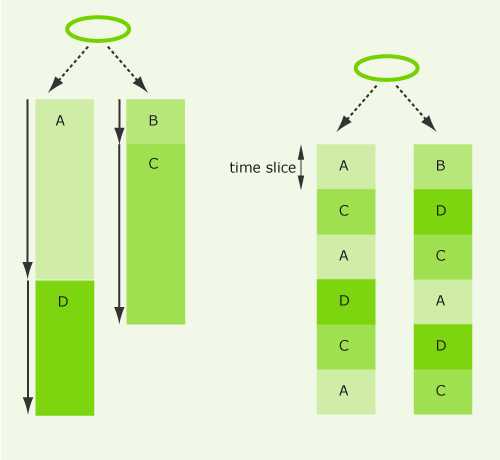
\includegraphics[width=0.6\linewidth]{img/process2.png}
\caption{Figure 2}
\label{fig:figure2}
\end{figure}

\subsection{\textit{Single vs. Multi-Threading}}
The process model discussed so far implies that by itself a process, consisting of a program being executed, only does one task at a time. We say that such process has a single thread of execution, or simply that the program is single threaded.\\\\
This limitation may sometimes be very undesirable for a program: for example, when a user action on a graphical interface requires a complex calculation, the user may not be willing to wait for the answer before doing something else. Several threads of execution are needed to allow parallel work in the program. We therefore say that such program is \textbf{multi threaded}.\\\\
Multi threaded programs are obviously better adapted to run on multi processor computers, in the same way that multi process environments are much more comfortable for the user experience on multi processor computers. But once again, such programs can also be executed on a single processor, requiring each thread to share the processor. We will assume that the means and rules to give the processor to a process can also be used inside a multi threaded programs to give the processor to a thread.

\subsection{\textit{Resources}}
To be executed, a process requires resources. There are different kinds of \textbf{resources}:
\begin{itemize}
\item hardware components of the computer, such as the processor, the memory, the hard drives, the mouse, the keyboard
\item logical components of the operating system, such as file for data storing or socket for network access
\end{itemize}
In the classical computer architecture, the main resources are the \textbf{processor}, \textbf{the memory}, the \textbf{hard drives}, and the other \textbf{IO devices}. In this module, we fill focus on means and rules to grant a process access to processor for some time \textbf{(CPU time)}. We will talk about the access to the memory in the \textit{Memory Management} module, the access to hard drives in the \textit{File System} module, and access to other IO devices in the \textit{Device Drivers and Input/Output module}.

\section{\textit{Processes}}
A program becomes a \textbf{process} as soon as it gets executed. A program is a passive entity, whereas a \textit{process} is an active entity, associated with a \textbf{program counter} specifying the next instruction to be executed and a set of resources that it requires. Multiple copies of the same program may be run simultaneously, each of them as a separate process. One user can invoke several copies of his/her web browser, or several users can open each their spreadsheet program. \\\\
An \textit{Operating System} can be seen as a \textbf{collection of processes}. During its whole life time, some processes exist from the time the system starts through the time it shutdowns while others are spawned when needed. A user may spawn a new process when clicking on an icon representing an instant messenger program, or a process can spawn at any time one or more new processes. \\\\
In normal circumstances, a process terminates when it finishes its task. A compiler stops when the target \textit{source code} is translated into \textit{object code}. A word processor stops when the user exits it. When an unexpected error occurs during the execution of a program, the process also terminates.

\subsection{Types and hierarchy}
We can classify processes in two types:
\begin{itemize}
\item \textbf{Foreground processes}, essentially users initiated processes
\item \textbf{Background processes}, essentially system processes devoted to common tasks, such as file printing, automated email retrieving. Such processes are often called \textbf{\textit{daemons}} under UNIX and \textbf{\textit{services}} under Windows
\end{itemize}
A process can spawn at any time a \textbf{child process}, which behaves like any other process. Under UNIX systems, the \textit{parent} and \textit{child} processes remains in a relational hierarchy, which implies some constraints. A parent process cannot terminate as long as any of its children are running. If a parent process is forced to terminate (killed), any of its children that are running are stopped at once. This is not the case under Windows, since a child process spawned by another process doesn't stay permanently in a hierarchical dependency with its parent.

\subsection{Process Control Block}
To manage the independent process model, it is necessary to have a special place in memory holding a \textbf{table of processes}. The table has an entry per process, called the \textbf{Process Control Block (PCB)}. Each entry keeps a number of information related to the process. We will discuss most of them in this module or in other modules.
\begin{figure}[!ht]
\centering
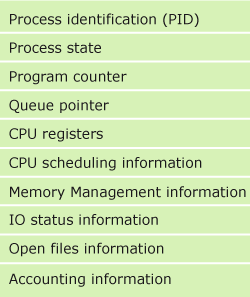
\includegraphics[width=0.35\linewidth]{img/PLB.png}
\caption{Figure 3}
\label{fig:figure3}
\end{figure}
\newpage
\subsection{Process states (life cycle)}
When a process is \textbf{created}, it is admitted into the table of processes with the state \textbf{\textit{new}}. At that time, there is no value for the program counter. As soon as the requested resources are identified and \textbf{allocated}, it is promoted to the state \textbf{\textit{ready}}.\\\\
The next step is the process to be granted access to the processor. This decision is made exclusively by a special program, the scheduler, which is implementing a scheduling algorithm as we will see later on. When access is granted, the process reaches the state \textbf{\textit{running}}. It is important to note, that at any given time only one process per processor can have the state running. The scheduler will take the process from the processor at the expiration of its time slot, making it fall back to the state \textbf{\textit{ready}}.\\\\
A running process might sometimes request some other resource or be blocked by another process. In those cases, it leaves the processor by itself and enters the state \textbf{\textit{waiting}}. It is now dependent on an event external to the processor. When that event occurs, the process will be promoted again to the state \textbf{\textit{ready}}. Finally a process that has completed its task goes to the state \textbf{\textit{terminated}}. Its associated PCB is deleted from the table of processes. \\\\
\begin{figure}[!ht]
\centering
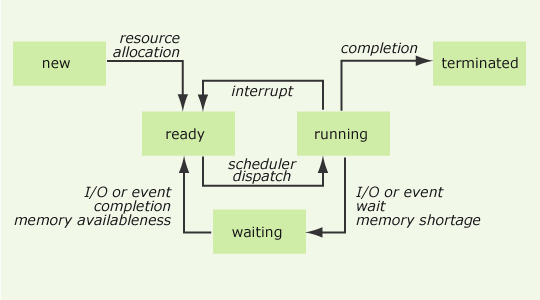
\includegraphics[width=0.8\linewidth]{img/states.png}
\caption{Figure 4}
\label{fig:figure4}
\end{figure}
From a logical point of view, it has to be noted that the two states ready and running are semantically equivalent. In both cases the process can be executed, however in the former case, the processor is temporarily unavailable.\\\\
On the other hand, the state \textbf{\textit{waiting}} implies that the process cannot be executed, even if the processor has nothing to do. Depending on the resource that is requested by the process, it finds itself in one of several kinds of waiting situation:
\begin{itemize}
\item \textbf{\textit{IO waiting (short term)}}. The process has to wait for an IO device to execute an action (i.e. reading from keyboard, writing to file) and subsequently producing an interrupt.
\item \textbf{\textit{Memory waiting (medium term)}}. The process has to wait for memory allocation, possibly requiring the memory management unit to initiate a page replacement.
\end{itemize}

\subsection{Context switching}
We saw that sometimes the scheduler might take a process from the processor, in particular when its time slot expires. In order for the process to restart from where it lefts the next time it is granted access to the processor, all necessary information must be saved. This is done by storing the program counter and all CPU registers in the PCB of the process. At the time the process is granted access to the processor again, the scheduler restores the program counter and the CPU registers in the processor, so that the process can continue its task where it stopped. This mechanism, called \textbf{context switching}, is illustrated in the next figure.
\begin{figure}[!ht]
\centering
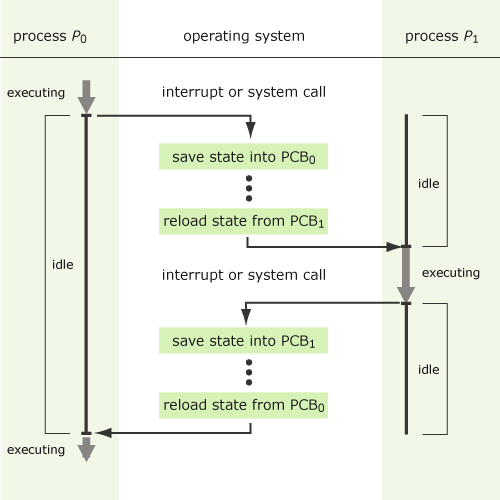
\includegraphics[width=0.6\linewidth]{img/context.png}
\caption{Figure 5}
\label{fig:figure5}
\end{figure}
It has to be noted that context switching is a time consuming mechanism. During the operation, the processor doesn't do any meaningful computation, it ist \textbf{idle}.
Thus, special attention must be given to the frequency of context switching. In particular if time slots get too small, the processor will spend most of its time switching from one process to another.

\subsection{Interruption}
An \textbf{interruption} is an unexpected event, breaking the sequential progression of a program. It can be emitted by a hardware component or even by the processor itself when an error occurs during the execution of an instruction. Normally, the running process is taken from the processor for the interrupt to be handled. The interruption mechanism will be covered in more details in the \textbf{Device Drivers and I/O module}.

\section{\textit{Multi Processor Architectures}}
As mentioned earlier, the general problematic is to grant \textbf{\textit{m}} simultaneous processes access to \textbf{\textit{n}} processors. In this chapter and in the next one, we will discuss solutions to achieve this goal restricting us to the case where we only have \textbf{\textit{one}} processor. These solutions can later be extended to \textit{multi processor} architectures.

\subsection{Objectives}
At this point we need to point to the difference between \textit{scheduling policies} and \textit{scheduling algorithms}. \textbf{Scheduling policies} are tightly tied to the objectives of a system and therefore can be arbitral; \textbf{scheduling algorithms} on the other hand are means to apply a policy and are defined as strict mathematical rules. \\\\
We can now differentiate two kinds of objectives. General objectives that apply in all situations and system dependent objectives that apply in specific situations, in which the system has particular requirements.
\paragraph{General Objectives} 
The idea is to maximize the global usage of the computer system and its components; different policies can be taken into consideration:
\begin{itemize}
\item \textbf{Optimizing CPU usage}, minimizing its idle time, i.e. periods during which the CPU has nothing to do.
\item \textbf{Maximizing the process throughput}, i.e. the number of processes that are granted access to the processor.
\item \textbf{Minimizing the turnaround time}, i.e. the time it takes for a process to go through all its states, from its creation (created state) to its death (terminated state).
\item \textbf{Minimizing the waiting time}, i.e. the time a process remains idle in the ready queue.
\end{itemize}

\paragraph{System dependent objectives}
These objectives can be strongly dependent on the characteristics of the system:
\begin{itemize}
\item \textbf{Real-time systems}. On such system, the policy is to \textit{guaranty} access to the processor each time a process needs it.
\item \textbf{Timesharing systems}. On such system, the policy is to \textit{optimize} the response time to the user.
\end{itemize}

\subsection{Approaches}
We have to distinguish between three scheduling approaches: \textbf{long term}, \textbf{medium term} and \textbf{short term}. The mechanisms are different for each of them; in particular the choice of a policy is driven by the objectives that need to be achieved. \\\\
\textbf{Long term scheduling} applies to programs, mostly daemons also known as background services, which need to run once at specified time or repeatedly with given recurrence (every hour, every day, every month, and so on). It is its responsibility to promote programs to the new state of a process when the system is not overloaded. This scheduler is not going to be discussed in this course since it does not present any special interest in the context of operating systems.\\\\
\textbf{Medium term scheduling} applies to processes, which require large amount of memory that cannot be granted at present time. It is its responsibility to swap out of the memory some processes to allow process in the \textit{waiting state} to be promoted to the \textit{ready state}. This scheduler is going to be discussed in the \textit{Memory Management} module. \\\\
\textbf{Short time scheduling} applies to processes that are in the \textit{ready state}. It is its responsibility to grant processor time to processes that need it. This scheduler is going to be discussed in the next chapter through the end of this module.

\section{\textit{Short time scheduler}}
The \textbf{short time scheduler} is a special program that selects among all ready processes the process that will be granted access to the processor. In case the time slot mechanism is in use, it also calculates the length of the time slot it will be given, depending on the number of other ready processes.

\subsection{Types and properties}
We have seen so far that at any given time aprocess is either using/requiring the processor, or waiting on some IOresources which when allocated will resume the process. Thus, a processexecution can also be defined as the strict alternating of CPU execution and IOwait, called respectively \textbf{CPU burst} and \textbf{IO burst}. Processes withlong CPU bursts and few IO bursts are said to be \textbf{CPU bound} while processes with a high rate of IO bursts and usually short CPU bursts are said to be \textbf{IO bound}.

\subsection{Pitfalls}
When developing a short time scheduler, we need to be aware of some common pitfalls and take them into consideration.
\begin{itemize}
\item \textbf{Starvation}. Starvation occurs when a process is never granted access to the processor. Several reasons could be source of starvation. Algorithms must be evaluated and proved against starvation.
\item \textbf{Context switching}. We can’t avoid this mechanism totally because it is the fundamental requirement to share the processor between processes. A process state transition to or from running involves context switching. It has to be considered as expansive as some CPU time is lost to non process computing activities. Algorithms have to take care of keeping context switching at minimum level.
\end{itemize}

\subsection{Queues}
The overall process scheduling is regulated by the use of \textbf{queues}. There are three types of queues.
\begin{itemize}
\item \textbf{Job queue}. Each newly created process is placed in the \textit{job queue}, associated with the state new. This queue contains all the processes in the system.
\item \textbf{Ready queue}. Each time a process is granted access to the memory and have obtained all necessary resources, it is placed in the \textit{ready queue}, associated with state \textit{ready}.
\item \textbf{Waiting queues}. When a process is not terminated and leaves the processor, it is placed in a \textit{waiting queue}, associated with the state \textit{waiting}. There are many kinds of waiting queues: \textit{wait for interrupt handling queues}, \textit{wait for child process termination queues} and \textit{device queues}. Each device has its own queue, with a name related to the type of the device: keyboard, screen, disk\# 0, disk\# 1, microphone, headset, terminal unit, and so on. Each time a process requires such a device, it is placed in the relevant \textbf{device queue}. \\\\
\end{itemize}
The \textit{ready queue} and the \textit{device queues} are implemented internally as \textit{linked lists}. Each element of the list is a Process ControlBlock (PCB) entry. The queue header holds pointers to the first and last PCBin the list. Each PCB holds a pointer to the next PCB in the queue, as shown in the figure \ref{fig:figure6}.
\begin{figure}[!ht]
\centering
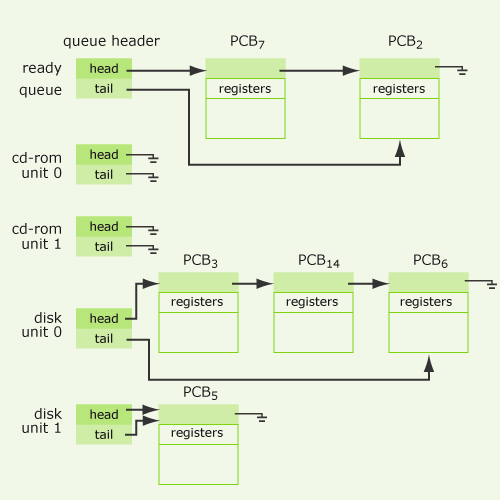
\includegraphics[width=0.7\linewidth]{img/Fig6.png}
\caption{Figure 6}
\label{fig:figure6}
\end{figure} \newpage
Queues are events driven. When a process releases a resource the first process in line in the corresponding queue isgranted access to it. If the later process now has been granted access to allrequested resources, it is placed back in the \textit{ready queue}. The \textit{processor} is associated with the \textit{ready queue}, and the \textit{hard drives} and other \textit{IO devices} with their own \textit{device queue}. In the remainder of this module, we will focus on the \textit{processor} and the \textit{ready queue}, leaving specific device queues mechanisms to be discussed in the \textit{Device Drivers and I/O} module.\\\\
When a process is granted access to the processor, because it has all requested resources, it is associated with the state \textit{running}. Such process doesn’t belong to the ready queue or to any device queue anymore. The process can now either finish, and be associated with the \textit{state terminated}, or leave the processor for numerous other reasons:
\begin{itemize}
\item The allocated time is over. The process is taken from the processor and is placed back in the ready queue, this mechanism is called \textbf{preemption}.
\item The process is interrupted. The process is taken from the processor and is placed back in the wait for \textit{interrupt handling queue}.
\item The process might request access to an IO device. The process leaves the processor and is placed in the \textit{device queue} of the corresponding device.
\item The process might spawn a new child process and wait for its termination. The process leaves the processor and is placed in the \textit{wait for child process termination queue}.
\end{itemize}
\begin{figure}[!ht]
\centering
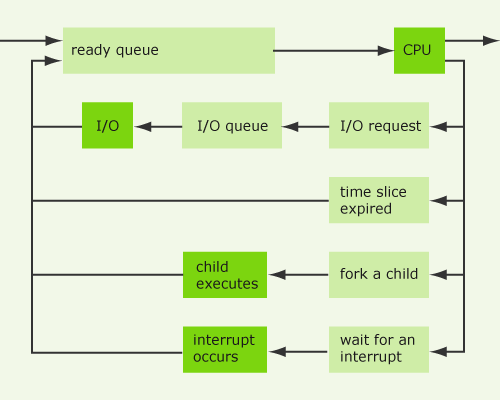
\includegraphics[width=0.8\linewidth]{img/Fig7.png}
\caption{Figure 7}
\label{fig:figure7}
\end{figure}
On \textit{time-sharing system}, there is also a medium term scheduler, responsible of sharing access to the memory. A process in the \textit{ready queue} can be swapped out to free memory and to allow another process to join the \textit{ready queue}. This approach can be viewed as an additional event, as shown in the next figure \ref{fig:figure8}.
\begin{figure}[!ht]
\centering
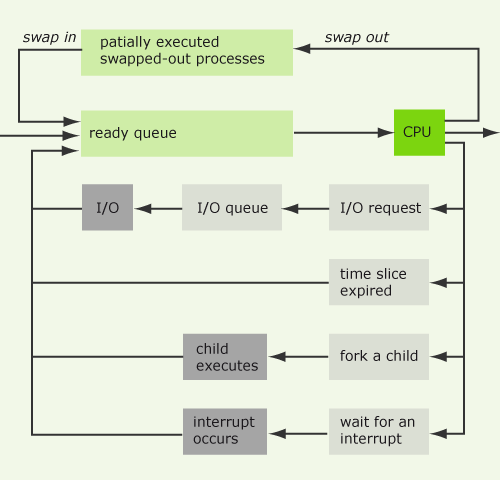
\includegraphics[width=0.8\linewidth]{img/Fig8.png}
\caption{Figure 8}
\label{fig:figure8}
\end{figure} \newpage

\subsection{Algorithms}
In this section, we will treat of algorithms that pick a process in the ready queue and give it to the processor. We will focus ourselves to the single processor case, since multi processors scheduling has the exact same problematic as soon as a process is dispatched to a processor. We will discuss the multi processor case later in this chapter. \\\\
Scheduling algorithms can be divided into two categories in respect to how they deal the allocation of processor time. A \textbf{non-preemptive} scheduling algorithm grants access to the processor for unlimited time. The process run until it finishes, blocks due to an IO request or blocks to wait for the termination of another process. A \textbf{preemptive} scheduling algorithm grants access to the processor for a limited time. If the process is still running when the allocated time is over, it is taken from the processor, placed back at the end of ready queue, and replaced by the next process in the ready queue.
\newpage
\paragraph{Non-preemptive algorithms}
\begin{itemize}
\item \textbf{First-Come-First-Served (FCFS)} \\
First-Come-First-Served algorithm is the most standard non-preemptive algorithm. Processes that request the CPU are granted access to the processor in order of arrival. This is simply accomplished by organizing the ready queue as a FIFO queue. When a new process arrives, its PBC is linked to the tail of the queue. \\\\
Let's consider that we have four processes arriving in the order P1, P2, P3 and P4 with run time of respectively 12, 6, 4 and 2 minutes. FCFS algorithm will run them in their order of arrival.
\begin{figure}[!ht]
\centering
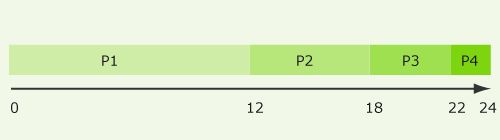
\includegraphics[width=0.7\linewidth]{img/Fig9a.png}
\caption{Figure 9a}
\label{fig:figure9a}
\end{figure}
We can calculate the waiting mean time (WMT) and the average turnaround time (ATT).
\begin{itemize}
\item WTM = (0 + 12 + 18 + 22)/4 = 13 minutes
\item ATT = (12 + 18 + 22 + 24)/4 = 19 minutes
\end{itemize}

\item \textbf{Shortest-Job-First (SJF)} \\
Shortest-Job-First algorithm is an alternative to FCFS. Processes that request the CPU are granted access to the processor starting with the shortest job. Let's go back to our previous example, we still have four processes arriving in the order P1, P2, P3 and P4 with run time of respectively 12, 6, 4 and 2 minutes. SJF algorithm will run them in the order P4, P3, P2 and P1.
\begin{figure}[!ht]
\centering
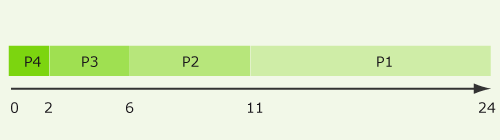
\includegraphics[width=0.7\linewidth]{img/Fig9b.png}
\caption{Figure 9b}
\label{fig:figure9b}
\end{figure}
We can again calculate the waiting mean time and the average turnaround time.
\begin{itemize}
\item WTM = (0 + 2 + 6 + 12) / 4 = 5 minutes
\item ATT = (2 + 6 + 12 + 24) / 4 = 11 minutes
\end{itemize}
We can see that SJF gives better results than FCFS and seems to be optimal. If the run time are a, b, c and d respectively, the average turnaround time is (4a + 3b + 2c+ d)/4. It is obvious that a contributes most, so to minimize the average turnaround time a should be the shortest job, b should be the next, then c and finally the longest job d as it affects only its own turnaround time. \\\\
However in the case the processes aren't arriving at the same time, and this is more realistic in common usage, SJF algorithm can give much worst results. It also requires the knowledge of the overall run time of each job, which also very often is not possible. Thus, SJF algorithm can hardly be used in modern systems.

\end{itemize}
\paragraph{Preemptive algorithms}
\begin{itemize}
\item \textbf{Round-Robin (RR)} \\
Round-Robin algorithm is the most standard \textit{preemptive} algorithm. It is based on FCFS algorithm, with the difference it artificially cuts the CPU time intoslices, called \textbf{time quanta}. As before, the \textit{ready queue} is organizedas a FIFO queue and whenever a new process arrives, its PBC is linked to the tail of the queue. \\\\
The processor is always granted to the first process in the queue but at most for a limited amount of time, and at this stage three scenarii can occur:
\begin{itemize}
\item The process may finish in the given quantum, and thus leaving the processor willingly and being associated with the state \textit{terminated}.
\item The process may, before the end of the quantum, be interrupted, request access to an IO device or spawn a new child process subsequently waiting for its termination, and thus leaving the processor willingly and being associated with the state \textit{waiting}.
\item The process may still have instructions to execute at the end of the quantum. The processor is taken away, and is given to the next process in line. Thus the former process still associated with the state \textit{ready} is placed back at the end of the \textit{ready queue} to take another share of the processor when its turn comes again.
\end{itemize}
As noted earlier, taking the processor from a running process at the end of a quantum and giving it to another is time consuming. The time used in context switching is lost in the sense the processor doesn’t do any meaningful computation. The performance of Round-Robin algorithm therefore heavily depends on the ratio of context switching length versus quantum length. For example, if we measure the context switching as 20 time units and the quantum is 100 time units, we can estimate that about 20\% of the CPU time is wasted. This could lead us to choose long quanta, so less time is wasted in context switching, but in this case the algorithm would becomes less and less preemptive degenerating into its base non-preemptive version FCFS. \\\\
The length of the \textit{quantum} is obviously influencing the performance of the system. A given quantum could minimize the waiting mean time, while another could minimize the average turnaround time. If quanta tend to be small, the system will have shorter response time giving the user a greater feeling of parallelism. As a rule of thumb, we can say that in \textit{time-sharing systems}, which widely make use of Round Robin algorithm, more than 50\% of the CPU bursts should be shorter than the quantum.

\item \textbf{Shortest-Remaining-Time-First (SRTF)} \\
Shortest-Remaining-Time-First algorithm is an improvement of SJF algorithm, which we remember rely solely on the overall run time of the jobs. We have seen earlier that processes strictly alternatebetween CPU bursts during which it needs the processor and IO bursts during which it waits for resource allocation. When a process that has been waiting on a resource is ready to resume, it is reintroduced in the \textit{ready queue}. At this stage, the remaining run time of the job has decreased. Furthermore if the scheduler is able to make an estimation of the length of the next CPU burst of such process, which is obviously less or equal than the remaining time of the job, it can also use this new information to elect the process with the shortest next CPU burst to be granted access to the processor. Note that so far this SRTF version is still non-preemptive letting processes run through the end of their CPU bursts. \\\\
The biggest issue remains, like in SJF, that in realistic environment the processes aren’t arriving at the same time and that early CPU bound processes can tie up the processor. SRTF is to reorder the ready queue each time a new process joins the queue or that a waiting process is resumed. If the first process in the \textit{ready queue} now has a shorter next CPU burst than the currently running process, the later is preempted and the processor is granted to the former. Thus we have a preemptive SRTF version, and we can see with the next example that it is more efficient than the non-preemptive version. \\\\
Let's consider that we have four processes. P1, arriving at 0 minute, has a run time of 7 minutes. P2, arriving at 2 minutes, has a run time of 4 minutes. P3, arriving at 4 minutes, has a run time of 1 minute. P4, arriving at 5 minutes, has a run time of 4 minutes. \\\\
Non preemptive SRTF will run them as follow.
\begin{figure}[!ht]
\centering
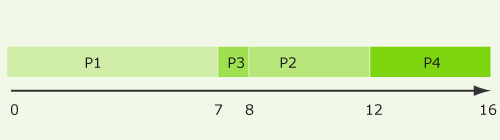
\includegraphics[width=0.65\linewidth]{img/Fig10a.png}
\caption{Figure 10a}
\label{fig:figure10a}
\end{figure}
We can calculate the waiting mean time (WMT) and the average turnaround time (ATT).
\begin{itemize}
\item WTM = (0 + 6 + 3 + 7)/4 = 4 minutes
\item ATT = (7 + 10 + 4 + 11)/4 = 8 minutes
\end{itemize}
Preemptive SRTF will run them as follow.
\begin{figure}[!ht]
\centering
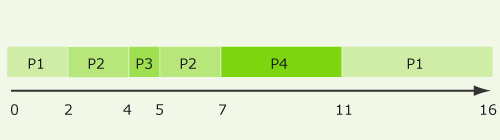
\includegraphics[width=0.65\linewidth]{img/Fig10b.png}
\caption{Figure 10b}
\label{fig:figure10b}
\end{figure}
We can again calculate the waiting mean time and the average turnaround time.
\begin{itemize}
\item WTM = ((0+9)+(0+1)+(0)+(2))/4 = 3 minutes
\item ATT = (16 + 5 + 1 + 6)/4 = 7 minutes
\end{itemize}

\item \textbf{Next CPU Burst Estimation} \\
As we have seen earlier, SFJ algorithm, as well as its SRTF improvement, is worth consideration since it has been shown to give optimal average turnaround times. However in order to be applicable it relieson an estimation of the overall run time of each job or at least of the length of the next CPU burst. \\\\
If we can make the assumption that the sequence of CPU burst and IO burst of a process is quite regular over its lifetime, we can approximate the length of the next CPU burst as being close to the previous ones. For the calculation, we use the following \textbf{exponential average formula} for the estimation of the length of the next CPU burst. \\\\
\begin{align}
\tau_{n+1} = \alpha \cdot t_n + (1 - \alpha ) \tau_n
\end{align}
where $t_n$ is the length of the last CPU burst, $\tau_n$ is the average of the length of past CPU bursts, and $\alpha$ is a tuning parameter in the range $[0; 1]$.\\\\
We can now discuss the value to give to $\alpha$.
\begin{itemize}
\item $\alpha = 0$, then $\tau_{n+1} = \tau_n = ... = \tau_0$. Only the first CPU burst is considered to be meaningful.
\item $\alpha = 1$, then $\tau_{n+1} = t_n$. Only the latest CPU burst is considered to be meaningful, we forget immediately about past history.
\item $\alpha = 0.5$. We average old and recent CPU bursts. As example, we estimate the sixth CPU burst as follow, $\tau_5 = 0.5 t_4 + (0.5)^2 t_3 + (0.5)^3 t_2 + (0.5)^4 t_1 + (0.5)^5 (t_0 + \tau_0)$, where $\tau_0$ is an arbitrary starting value statistically given by typical processes. We notice the decreasing importance of old CPU burst in the average over time. This is known as aging average, which often is used when prediction must be made on the basis of previous measurement.
\end{itemize}

The formula becomes the following:

\begin{align}
\tau_{n+1} = \frac{(t_n + \tau_n)}{2}
\end{align}

\item \textbf{Priority Scheduling} \\
We can also associate with each process a notion of priority. The implicit scheduling policy requires that a higher priority process has to be run before a lower priority process. So far FCFS and RR can be considered as equal priority scheduling, while SJF and SRTF can be considered as priority scheduling, with an associated priority defined as the inverse of the overall run time respectively the next CPU burst. \\\\
But in most cases priorities are system or user specified. Processes can be categorized in groupsaccording to their importance in the system. For example, we can have systemprocesses which ensure the fundamental functionalities of the system, interactive processes which are IO driven, service processes which provide additional functionalities and computation processes which are CPU driven. Each group is assigned a priority level, with an associated quantum and its own \textit{ready queue}, and at any given priority level processes are treated sequentially using Round-Robin algorithm. As long as a process stays in a higher level ready queue, processes in a lower level \textit{ready queue} are not granted access to the processor. This has the major drawback that it can lead to \textbf{starvation} (also known as \textbf{indefinite blocking}). \\\\
Solutions have been developed though to make this class of algorithms usable. One idea is to allow the priority of a process to dynamically change over time adjusting itself based on different criteria. In order to illustrate this, let’s consider having \textit{P} priorities, ranging from \textit{0} being the lowest to \textit{P-1} being the highest, each of them having their own \textit{ready queue}. When a process is created, it is associated with a priority, its \textbf{nominative priority}, depending on its nature and placed in the corresponding level \textit{ready queue}. During the entire lifetime of a process, its priority can be increased or decreased according to specific criteria through events, moving the process up or down within some part or even the whole queue hierarchy. At this stage it has to be kept in mind that system processes should always have a higher priority than user processes. \\\\
Firstly preemption could force the process priority to be decreased by one or more units. Converselythe passing of time could slowly increase the priority of each ready by a given amount, this mechanism being known as an \textbf{aging}. Furthermore whenever a process re-enters the \textit{ready queue}, for example after the completion of an IO request, it could do it at its nominative priority, at its latest running priority (the priority it had at the time it left the processor), or at a priority directly proportional to the unused percentage of its last running quantum making place to complex policies and optimizations. It has to be noted, as a final consideration, that process priorities could be used not only to order the \textit{ready queue} but also other \textit{device queues} making devices more easily available to higher level processes.
\end{itemize}

\subsection{Multiprocessor}
We have seen in the introduction that multi tasking can obviously take advantage of multiprocessor computers, which allows morethan one process to be executed simultaneously. However on such systems the improved efficiency comes at the cost of more complex scheduling decisions, especially in the case of some device belonging exclusively to a givenprocessor. \\\\
We distinguish two types of multiprocessor architectures: \textbf{symmetric} and \textbf{asymmetric}. In a symmetric multiprocessor (SMP), also known as a homogenous system, all processors areidentical. Each processor is said to be \textbf{self-scheduling}, which mean it alones makes all scheduling decisions. In an asymmetric multiprocessor (AMP), however, one processor, called the \textbf{master processor}, takes the responsibility of all system tasks and specifically of all scheduling decisions dispatching the processes to the otherprocessors, called the \textbf{slave processors}, which are solely devoted to execute user (non system) tasks. Now, as we remember our first general objective is to optimize CPU usage, let’s observe more closely how it relates to the two types of architectures. \\\\
On a symmetric multiprocessor (SMP), each process whether system or user can be executed on any processor. There are different approaches to scheduling in such context. A \textit{common ready queue} can be shared by all processors, or a common controller can dispatch, possibly depending on the current load on each processor, the process to the \textit{private ready queue} of the processor on which it will stay during its entire lifetime. \\\\
On an asymmetric multiprocessor (AMP), each user process can be executed on any \textit{slave processors}. The \textit{master processor} manages a \textit{single ready queue} similarly to what have been discussed in earliersections. Processes are granted access, in the order of the queue, to the \textit{slave processors} as they become free. Thus the load on each processor is inherently \textbf{balanced}. If it occurs that a process must be executed on aprocessor having specific characteristics, the \textit{master processor} additionally manage a \textit{ready queue} for each subset of processors sharing the same characteristics. \\\\
In SMP architecture with a \textit{common ready queue} or in AMP architecture, a process might be executed on one processor, leave it after being preempted or making an IO request, and resume later on another processor. In this situation, known as \textbf{process migration}, \textit{context switching} gets more expansive, since the cache of the newly used processor needs to be populated with data that is to be invalidated in the cache of the former processor. To retain efficiency, scheduling algorithms aim to associate a process with its most recent used processor, possibly making itwait a little bit longer in the \textit{ready queue} in order to minimize or even avoid \textit{process migration}. This is known as \textbf{processor affinity}. We can observe however that this policy opposes to the \textbf{load balancing} policy, which we remember aim to distribute the work evenly among all processors. Thus there is no absolutely best solution, and a trade-off mainly depending on hardware considerations and on the nature of the processes in the system need to be set.

\section{\textit{Readings section}}
You have now reached the readings section that is subdivided into required and recommended readings. \\\\
Required readings are articles taken out of real life, originating from the area of the theory section. 
Recommended readings are interesting and fit the theory but are not a must; they are intended for people more interested into the study matter. \\\\
With these readings you get used to the style of scientific writting. \\\\
It is not easy to read and understand scientific articles. If you start reading with the abstract you get an overview of the work presented. The introduction leads to the presented facts and helps understanding them. The most important section is the discussion. That is where the gained results are brought into context.

\subsection{Books}
\begin{itemize}
\item Abraham Silberschatz, Peter Baer Galvin, Greg Gagne: Operating System Concepts, 7th Edition 2005,
John Wiley \& Sons, Inc.; ISBN 0-471-69466-5 \\
\textit{Part two - Process Managment, Chapter 3 \& Chapter 5} 
\item Andrew S. Tanenbaum: Modern Operating Systems, 2nd Edition 2001, Prentice Hall, Inc.; ISBN 0-13-092641-8 \\
\textit{Chapter 2 - Porcesses and threads, Section 2.1 \& Section 2.5}
\end{itemize}

\section{\textit{Self Test}}
The Self Test helps you to decide whether you are ready for the Quiz or not. In case of wrong answers you get links to additional information where you can improve your knowledge. The Self Test is not reviewed. It is for your personal use and benefit only. \\\\
You can start the Self Test by following \href{https://ilias.unibe.ch/ilias.php?baseClass=ilObjTestGUI&ref_id=402563&cmd=infoScreen}{this link} and clicking on the \textit{''Start the Test''} button.
There are no time limitations to this task and you can always come back. \\\\
Evaluation criteria: 
No points can be earned for this task.

\section{\textit{Quiz}}
If you feel ready for the hands-on session and you are satisfied with your Self Test results, solve the Quiz. The Quiz results will be reviewed and evaluated by your tutor.
You must finish the Quiz before proceeding to the hands-on session! \\\\
You can start the Quiz by following \href{https://ilias.unibe.ch/ilias.php?baseClass=ilObjTestGUI&ref_id=402568&cmd=infoScreen}{this link} and clicking on the \textit{''Start the Test''} button.
There are no time limitations to this task and you can always come back. \\\\
Evaluation criteria:
You can earn a total of 20 points for this task and each question gives a certain amount of points.

\chapter{Knowledge Application/Exploration}
\section{Simulator Overview}
In this section, we will introduce you to the simulation engine that you will use for the hands-on session of this module. The UniNE Process Scheduling Simulator is a Java program that is designed to run virtual processes in an environement consisting of virtual devices. It also gathers information throughout its execution in order to allow the computation of pertinent statistics.
\begin{itemize}
\item \textbf{Virtual devices} - A virtual device actually represent an hardware device in a real system. This can be any IO device, such as an hard disk, or another media device such as a Floppy drive, a CD/DVD drive or a Network controller.
\item \textbf{Virtual processes} - A virtual process actually represent a process in a real system. The virtual process starts its life upon its creation, which can occur at any time. The virtual process is then in turns either requiring the processor, for a variable amount of time, or requesting any IO device existing in the environement, also for a variable amount of time. The last stage of a virtual process is its termination, which occur after it has completed its last instruction.
\end{itemize}

\section{Simulator Components}
Here we will introduce you to the three interfaces that you will have to know in order to make use of our simulation engine.\\\\
The \textit{Kernel} interface is the core interface of the UniNE Process Scheduling Simulator. It represents the scheduler consisting of system call handlers and interrupt handlers that are to be called by the simulation engine at specific times on the basis of the life cycles of all the processes in to the system. It is made of the following methods: 
\begin{itemize}
\item void systemCallInitIODevice(String deviceID, Simulator simulator) - This system call is issued once for each device listed in the devices file specifiedon the command line when the Simulator is executed.
\item void systemCallProcessCreation(String processID, long timer, Simulator simulator) - This system call is issued once for each process, at the process' arrival time as specified in its data file. This system call indicates the arrival of the process in the system.
\item void systemCallProcessTermination(long timer, Simulator simulator) - This system call is issued once for each process, once the process has completed its execution.
\item void systemCallIORequest(String deviceID, long timer, Simulator simulator) - This system call is issued each time a user process requests an I/O Operation. Note that any requests for operations on devices that do not exist should cause the program to terminate with an error message.
\item void interruptIODevice(String deviceID, long timer, Simulator simulator) - This interrupt may arrive from any I/O device created by a InitIODevice system call. If an interrupt arrives from any other device the scheduler should cause the program to terminate with an error message.
\item void interruptPreemption(long timer, Simulator simulator) - This interrupt may arrive when preemption occurs.
\item String running(long timer, Simulator simulator) - This method returns the name of the process currently in the running state. When no other process is ready to run the Kernel must report that the "Idle" process is running.
\item void terminate(long timer, SimulatorStatistics simulator) - This method is called when the simulation has completed. The code in this method should compute statistics and display the results of the simulation.
\end{itemize}
The \textit{Simulator} interface provides you simple means to interact with the simulation engine. The following methods are designed to be used in any system call handler or interrupt handler:
\begin{itemize}
\item boolean schedulePreemptionInterrupt(long delay) - Schedule a timer interrupt to occur after the specified number of time units. The timer is set to begin when the system call that started it completes. Thus a process started to run when a timer is set will be allowed to run for a full ''delay'' time units.
Only one timer interrupt can be scheduled at a time. If the event queue already contains a timer interrupt that timer interrupt will be canceled and a new one created.
\item boolean cancelPreemptionInterrupt() - Cancel a timer interrupt if one has been set. If a timer interrupt has been set, it is removed from the event queue. If no timer interrupt has been set this method does nothing.
\item long queryOverallTime(String processID) - Query the overall time of a given process. If the process exists, its overal time is returned. If the process does not exist, the value -1 is returned.
\item long queryBurstRemainingTime(String processID) - Query the remaining time of the current burst of a given process. If the process exists, its remaining time of the current burst is returned. If the process does not exist, the value -1 is returned.
\end{itemize}

The \textit{SimulatorStatistics} interface provides you simple means to retrieve information from the simulation engine.The following methods aredesigned to beused specifically in Kernel's terminate method:
\begin{itemize}
\item long getSystemTime() - Return the current system time. This is the total number of virtual time units that have elapsed since the system has started. It should agree with the value obtained from getUserTime() + getIdleTime()
\item long getUserTime() - Return the current user time. This is the number of virtual time units that the system has spent performing user operations.
\item long getIdleTime() - Return the current idle time. This is the number of virtual time units that the system has spent executing the idle process.
\item int getSystemCallsCount() - Return the current system calls count. This is the number of time the simulator has called a Kernel method.
\item void formatStatistics(PrintStream stream, long system, long user, long idle, int calls, int saves, long wmt, long att) - Print statistics. This is the method to call with yourvalues to nicely print out the statistics. \textit{System.out} should be used as the first formal parameter.
\end{itemize}

\section{\textit{First Come/First Serve}}
\subsection{Tasks}
\begin{itemize}
\item You have to implement the \textit{Kernel} interface for a First Come/First Serve scheduler.
\item You have to print the overall systemTime, userTime and idleTime and compute the CPU usage.
\item You have to print the overall system call count.
\item You have to calculate the register saves count.
\item You have to compute the average turnaround time (ATT).
\item You are to compute the waiting mean time (WMT).
\end{itemize}

\subsection{Indication}
In Kernel's terminate method, you are to call SimulatorStatistics' formatStatistics method with appropriate parameters in orderto print all statistics in a standard way. The output ought to be similar to the following: \\\\
System Time: 24 [100.00\%]\\
User Time: 24 [100.00\%]\\
Idle Time: 0 [0.00\%]\\\\
System Calls: 8\\
Registers Saves: 0\\\\
Av. Turnaround Time: 19.0\\
Wait Mean Time: 13.0\\\\
HINT: Some parameters can be received from the SimulatorStatistics class.

\subsection{Submission}
In order to complete this task, you will be using the \href{https://oslab.unine.ch/portal/modules/0/oslab.jsp}{OSLab Hands-On applet}. You will use this applet to write your code, compile it, debug it and run an automated evaluation procedure. You will be required to successfully pass the automated evaluation procedure in order to receive a fingerprint that you will be asked to copy and paste to the appropriate field in the Final Quiz of the module.

\subsection{Evaluation}
The OSLab Hands-On applet will run your implementation of the scheduler with a randomized set of virtual devices and processes and automatically check your output for correctness against our reference implementation. Your tutor will also evaluate your coding style.

\section{\textit{Round Robin}}
\subsection{Tasks}
\begin{itemize}
\item You have to implement the Kernel interface for a Round Robin scheduler with a time slice of 2.
\item You have to print the overall systemTime, userTime and idleTime and compute the CPU usage.
\item You have to print the overall system call count.
\item You have to calculate the register saves count.
\item You have to compute the average turnaround time (ATT).
\item You have to compute the waiting mean time (WMT).
\end{itemize}

\subsection{Indication}
We consider that a preemption occurs a full time slice delay after a process started running. If the process leaves the CPU before the expiration of the time slice, this preemption is canceled.\\\\
In Kernel's terminate method, you are to call SimulatorStatistics' formatStatistics method with appropriate parameters in orderto print all statistics in a standard way. The output ought to be similar to the following:\\\\
System Time: 24 [100.00\%]\\
User Time: 24 [100.00\%]\\
Idle Time: 0 [0.00\%]\\\\
System Calls: 14\\
Registers Saves: 6\\\\
Av. Turnaround Time: 16.0\\
Wait Mean Time: 10.0\\\\
HINT: Some parameters can be received from the SimulatorStatistics class.

\subsection{Submission}
In order to complete this task, you will be using the \href{https://oslab.unine.ch/portal/modules/3/}{OSLab Hands-On applet}. You will use this applet to write your code, compile it, debug it and run an automated evaluation procedure. You will be required to successfully pass the automated evaluation procedure in order to receive a fingerprint that you will be asked to copy and paste to the appropriate field in the Final Quiz of the module.

\subsection{Evaluation}
The OSLab Hands-On applet will run your implementation of the scheduler with a randomized set of virtual devices and processes and automatically check your output for correctness against our reference implementation. Your tutor will also evaluate your coding style.

\section{\textit{Shortest Remaining Job First (preemptive)}}
\subsection{Tasks}
\begin{itemize}
\item You have to implement the Kernel interface for a \textbf{preemptive} Shortest Remaining Job First scheduler.
\item You have to print the overall systemTime, userTime and idleTime and compute the CPU usage.
\item You have to print the overall system call count.
\item You are to calculate the register saves count.
\item You have to compute the average turnaround time (ATT).
\item You have to compute the waiting mean time (WMT).
\end{itemize}

\subsection{Indication}
In Kernel's terminate method, you are to call SimulatorStatistics' formatStatistics method with appropriate parameters in orderto print all statistics in a standard way. The output ought to be similar to the following:\\\\
System Time: 24 [100.00\%]\\
User Time: 24 [100.00\%]\\
Idle Time: 0 [0.00\%]\\\\
System Calls: 8\\
Registers Saves: 3\\\\
Av. Turnaround Time: 11.0\\
Wait Mean Time: 5.0\\\\
HINT: Some parameters can be received from the SimulatorStatistics and the Simulator classes.

\subsection{Submission}
In order to complete this task, you will be using the \href{https://oslab.unine.ch/portal/modules/2/oslab.jsp}{OSLab Hands-On applet}. You will use this applet to write your code, compile it, debug it and run an automated evaluation procedure. You will be required to successfully pass the automated evaluation procedure in order to receive a fingerprint that you will be asked to copy and paste to the appropriate field in the Final Quiz of the module.

\subsection{Evaluation}
The OSLab Hands-On applet will run your implementation of the scheduler with a randomized set of virtual devices and processes and automatically check your output for correctness against our reference implementation. Your tutor will also evaluate your coding style.

\end{document}

